%!TEX root = ../these.tex

В машиностроении, производстве металлоконструкций и
многих других отраслях промышленности значительная часть продукции
производится из заготовок, получаемых из листовых материалов.
В процессе планирования производства
на предприятиях используются отечественные и зарубежные
системы автоматизированного проектирования (САПР),
предназначенные для разработки управляющих программ (УП)
для машин листовой резки с ЧПУ
(числовым программным управлением).
Хотя они позволяют автоматизировать разработку УП,
на зачастую не способны решать оптимизационные задачи.
По этой причине
пользователям САПР
в процессе проектирования маршрута инструмента
зачастую приходится использовать интерактивные методы проектирования
УП,
поскольку алгоритмы автоматической генерации УП
во многих случаях не позволяют генерировать
оптимальные управляющие программы,
а также обеспечивать соблюдение технологических требований листовой резки.

В качестве критериев
оптимизации обычно используются длительность процесса листовой резки и его стоимость.
Проблема разработки методов, алгоритмов
и соответствующего программного обеспечения,
позволяющих оптимизировать параметры процесса резки заготовок
из листовых материалов на машинах с ЧПУ
в неинтерактивном режиме,
включая сюда также алгоритмы маршрутизации движения инструмента,
которые бы обеспечивали минимизацию времени резки и стоимости процесса,
остается актуальнейшей задачей для раскройно-заготовительного производства.

\begin{figure}
  \centering
  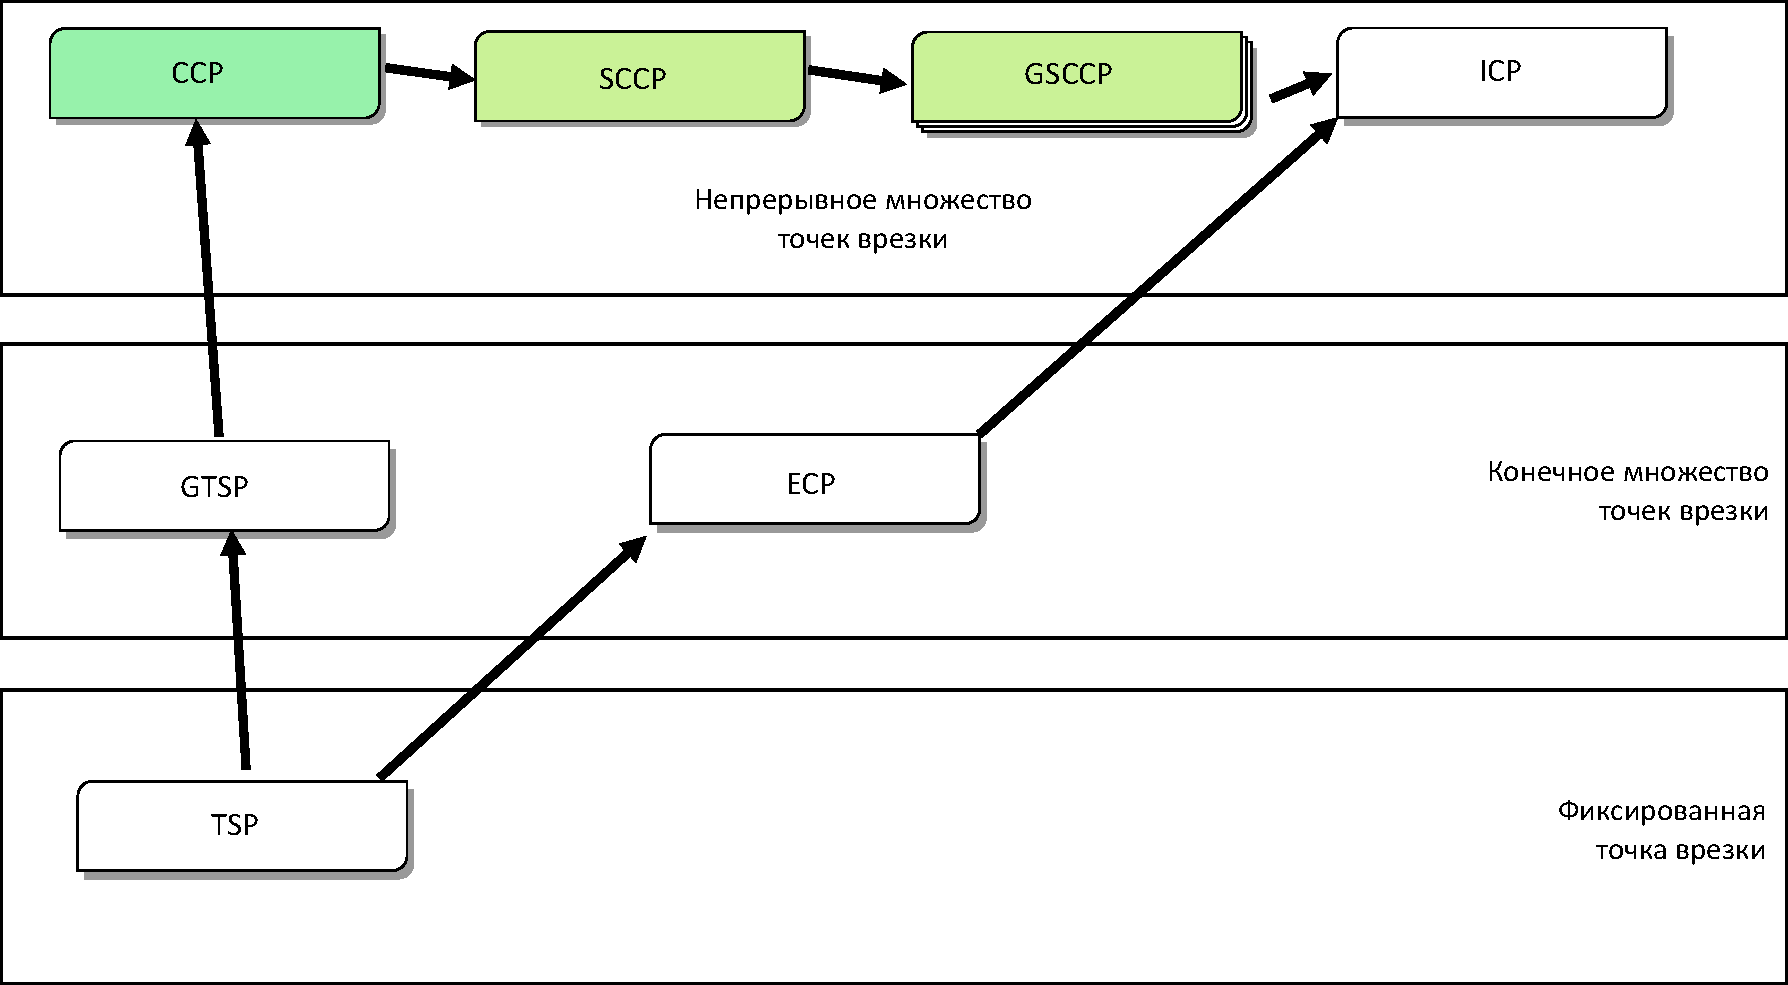
\includegraphics[width=0.95\textwidth]{classes.pdf}
  \caption{Классификация задач резки}
  \label{fig:cut-classes}
\end{figure}
